\documentclass{article}

\usepackage{polski}
\usepackage[utf8]{inputenc}
\usepackage{graphicx}
\usepackage{amsfonts}
\usepackage{amssymb}
\usepackage{amsmath}
\usepackage{listings}
\usepackage{breqn}
\usepackage{float}

\author{Maciej Pieta \and Piotr Koproń \and Jakub Woś \and Rafał Piwowar}
\date{Marzec 2023}

\title{Technika Cyfrowa. \\ Ćwiczenie 3.}

\begin{document}
\maketitle
\newpage
\section{Zadanie 3a}
\paragraph{Treść zadania.}
Bazując na dowolnie wybranych przerzutnikach, zaprojektować, zbudować i przetestować synchroniczny trzybitowy licznik liczący w następujący sposób:
     0, 2, 4, 6, 1, 3, 5, 7, 0, 2 , 4 , … itd.
Inaczej mówiąc: licznik najpierw przechodzi po wartościach parzystych, a potem po wartościach nieparzystych, i znowu po parzystych, i tak w kółko.
\subsection{Ogólna idea rozwiązania}
\begin{figure}[H]
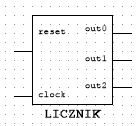
\includegraphics[width = 0.5\textwidth]{3a_blackbox}
\end{figure}
Licznik jest trzybitowy - wartość wyjściowa jest definiowana jako $1*out_{0}+2*out_{1}+4*out_{2}$.
Jako wartości wejściowe przyjmujemy zewnętrzny zegar oraz sygnał resetujący.
\subsection{Tabele prawdy}
Tabele prawdy informują o kolejnej wartości wysyłanej przez licznik, wyznaczone z wartości aktualnej.
\begin{figure}[H]
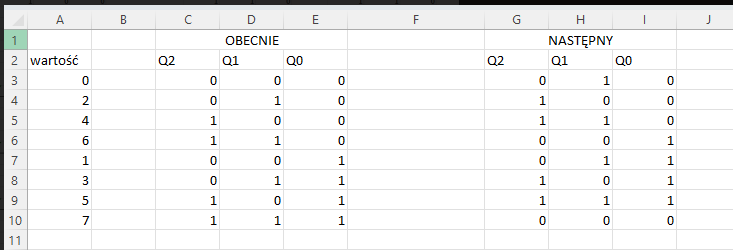
\includegraphics[width = \textwidth]{3a_tabele_prawdy}
\end{figure}
\subsection{Tabele Karnaugh}
Dokonujemy minimalizacji, w celu wyznaczenia bezpośrednich wzorów na kolejne wartości, oznaczone $D_{0}, D_{1},D_{2}$.
\begin{figure}[H]
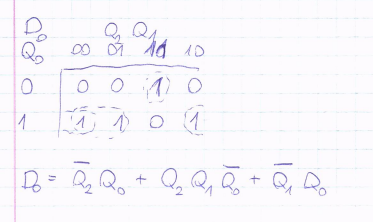
\includegraphics[width = 0.5\textwidth]{3a_karnaugh_2}
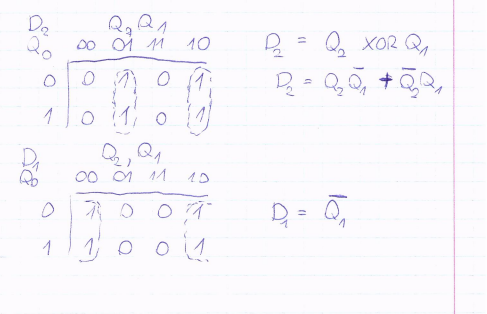
\includegraphics[width = 0.5\textwidth]{3a_karnaugh_1}
\end{figure}
\subsection{Schemat układu}
\begin{figure}[H]
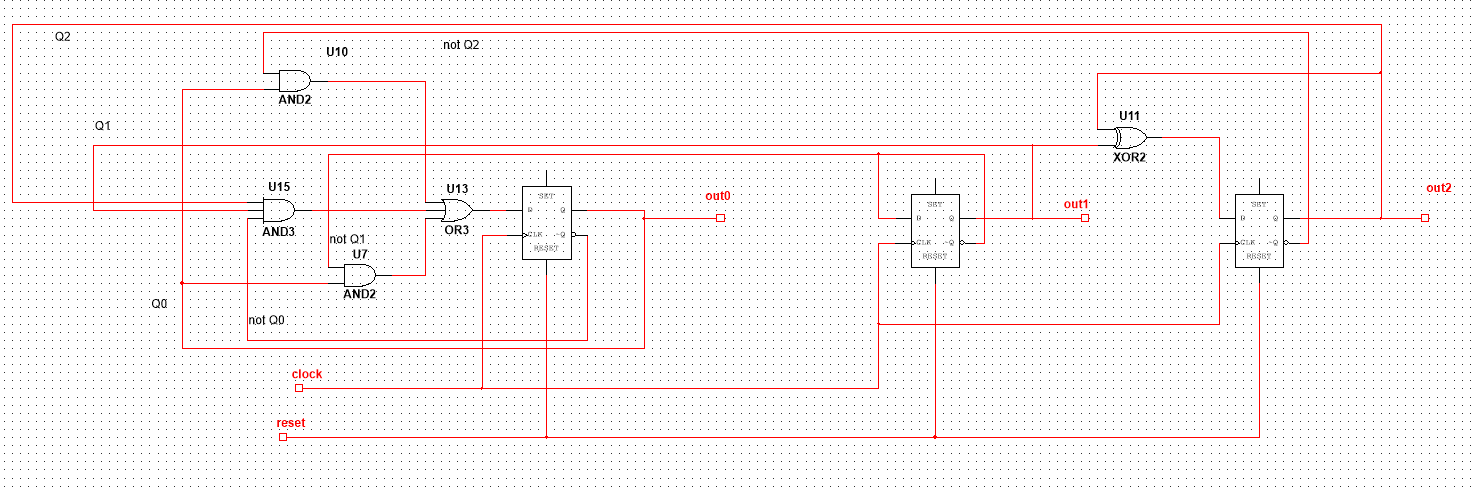
\includegraphics[width = \textwidth]{3a_uklad}
\end{figure}
Dodatkowo załączamy układ wizulalizacjy działanie naszego licznika.
\begin{figure}[H]
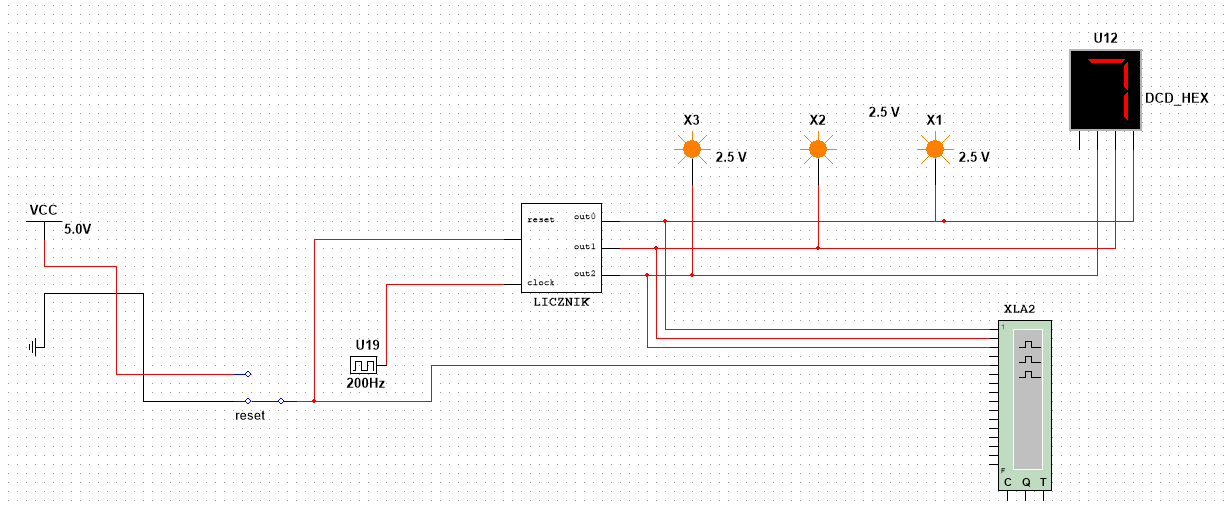
\includegraphics[width = \textwidth]{3a_wizualizacja}
\end{figure}
\subsection{Układ testujący}
Przygotowaliśmy automatyczny model testujący. Lampka błędu pozostanie zgaszona tylko jeżeli we wszystkich sytuacjach licznik zachowa się zgodnie z oczekiwaniami.
\begin{figure}[H]
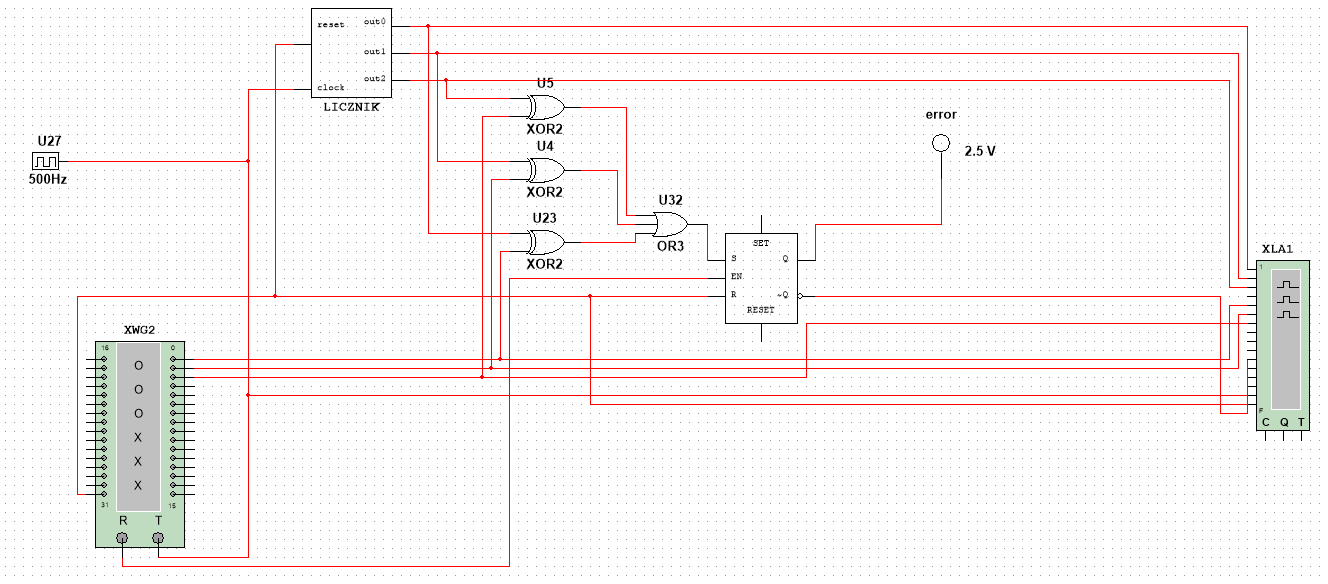
\includegraphics[width = \textwidth]{3a_tester}
\end{figure}
Ustawienia generatora słów i wyniki analizatora logicznego.
\begin{figure}[H]
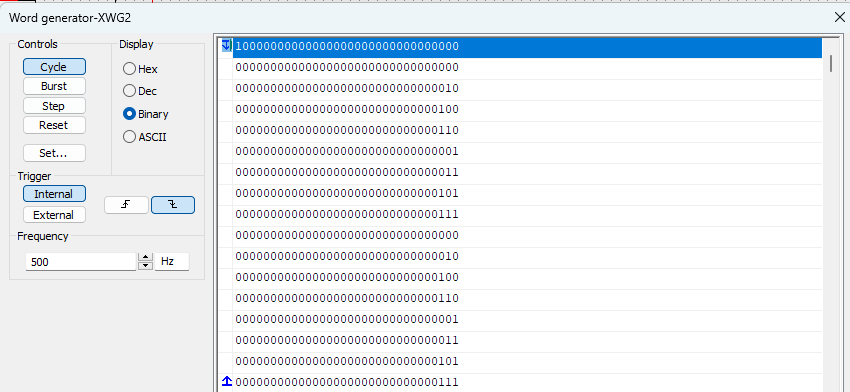
\includegraphics[width = \textwidth]{3a_generator}
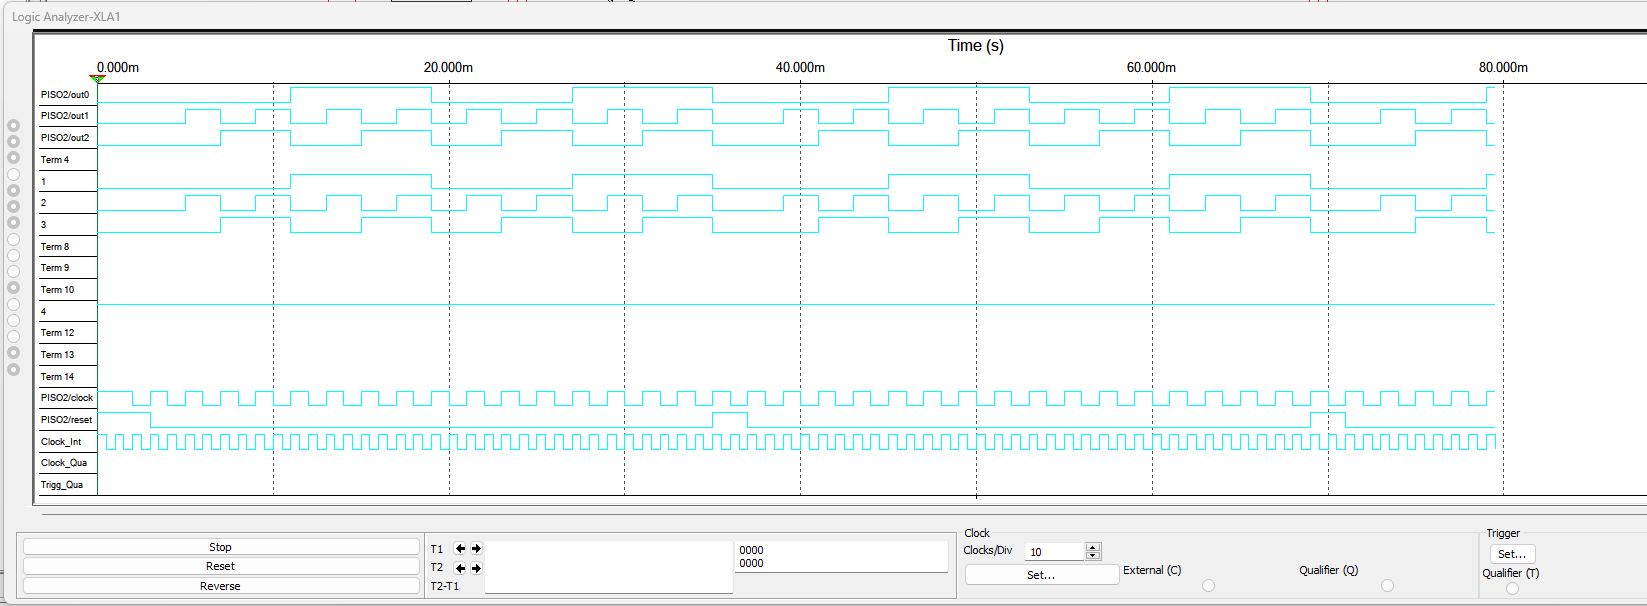
\includegraphics[width = \textwidth]{3a_analizer}
\end{figure}
Wartość oznaczona "4" stale ja 1 oznacza że lampka błędu nie świeci, czyli program działa.
\subsection{Wnioski}
\paragraph{Alternatywne rozwiązania}
\paragraph{Zastosowania}
Licznik może być wykorzystany do synchronizacji sygnalizacji świetlnej interskrzyżowaniowo, w celu zapewnienia optymalnych warunków jazdy dla kierowców jadących zgodnie z ogarniczeniami prędkości. (Jak jedzie przepisowo, to cały czas będzie miał zielone, jak nie - to i tak będzie musiał hamować na czerwonym).
RYSUNEK DO TEGO.
\section{Zadanie 3b}
\paragraph{Treść zadania}
Bazując na przerzutnikach "D", zaprojektować, zbudować i przetestować automat realizujący detekcję wprowadzanej na jego wejście czterobitowej wartości. Automat powinien rozpoznawać liczbę binarną: "1101". Jako źródło wprowadzanej wartości proszę użyć układu zbudowanego w ramach ćw.2b.
\paragraph{Układ zbudowany w ramach ćwiczenia 2b}
Zgodnie z komentarzem zwrotnym do ćwiczenia 2b, zbudowany przez nas układ PISO wymagał pewnych poprawek. Dla klaryfikacji, załączamy tutaj poprawioną wersję.
\begin{figure}[H]
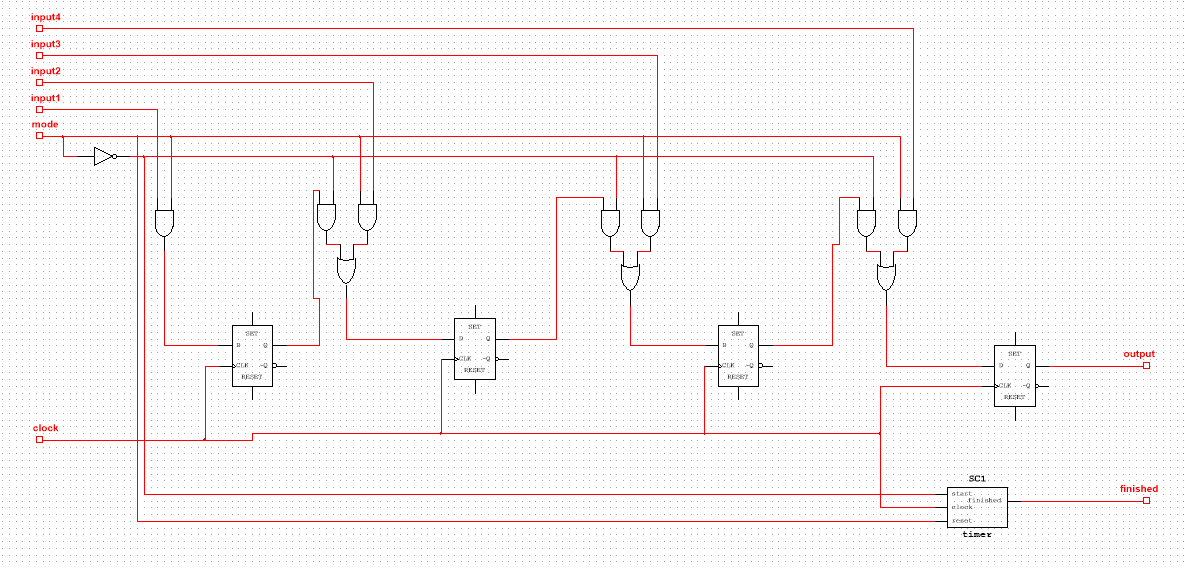
\includegraphics[width = \textwidth]{3b_2b_klaryfikacja}
\end{figure}
\subsection{Ogólna idea rozwiązania}
FIXME: Add Wejścia/Wyjścia.
\begin{figure}[H]
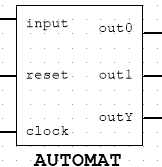
\includegraphics[width = 0.5\textwidth]{3b_blackbox}
\end{figure}
Implementujemy następujący automat:
\begin{figure}[H]
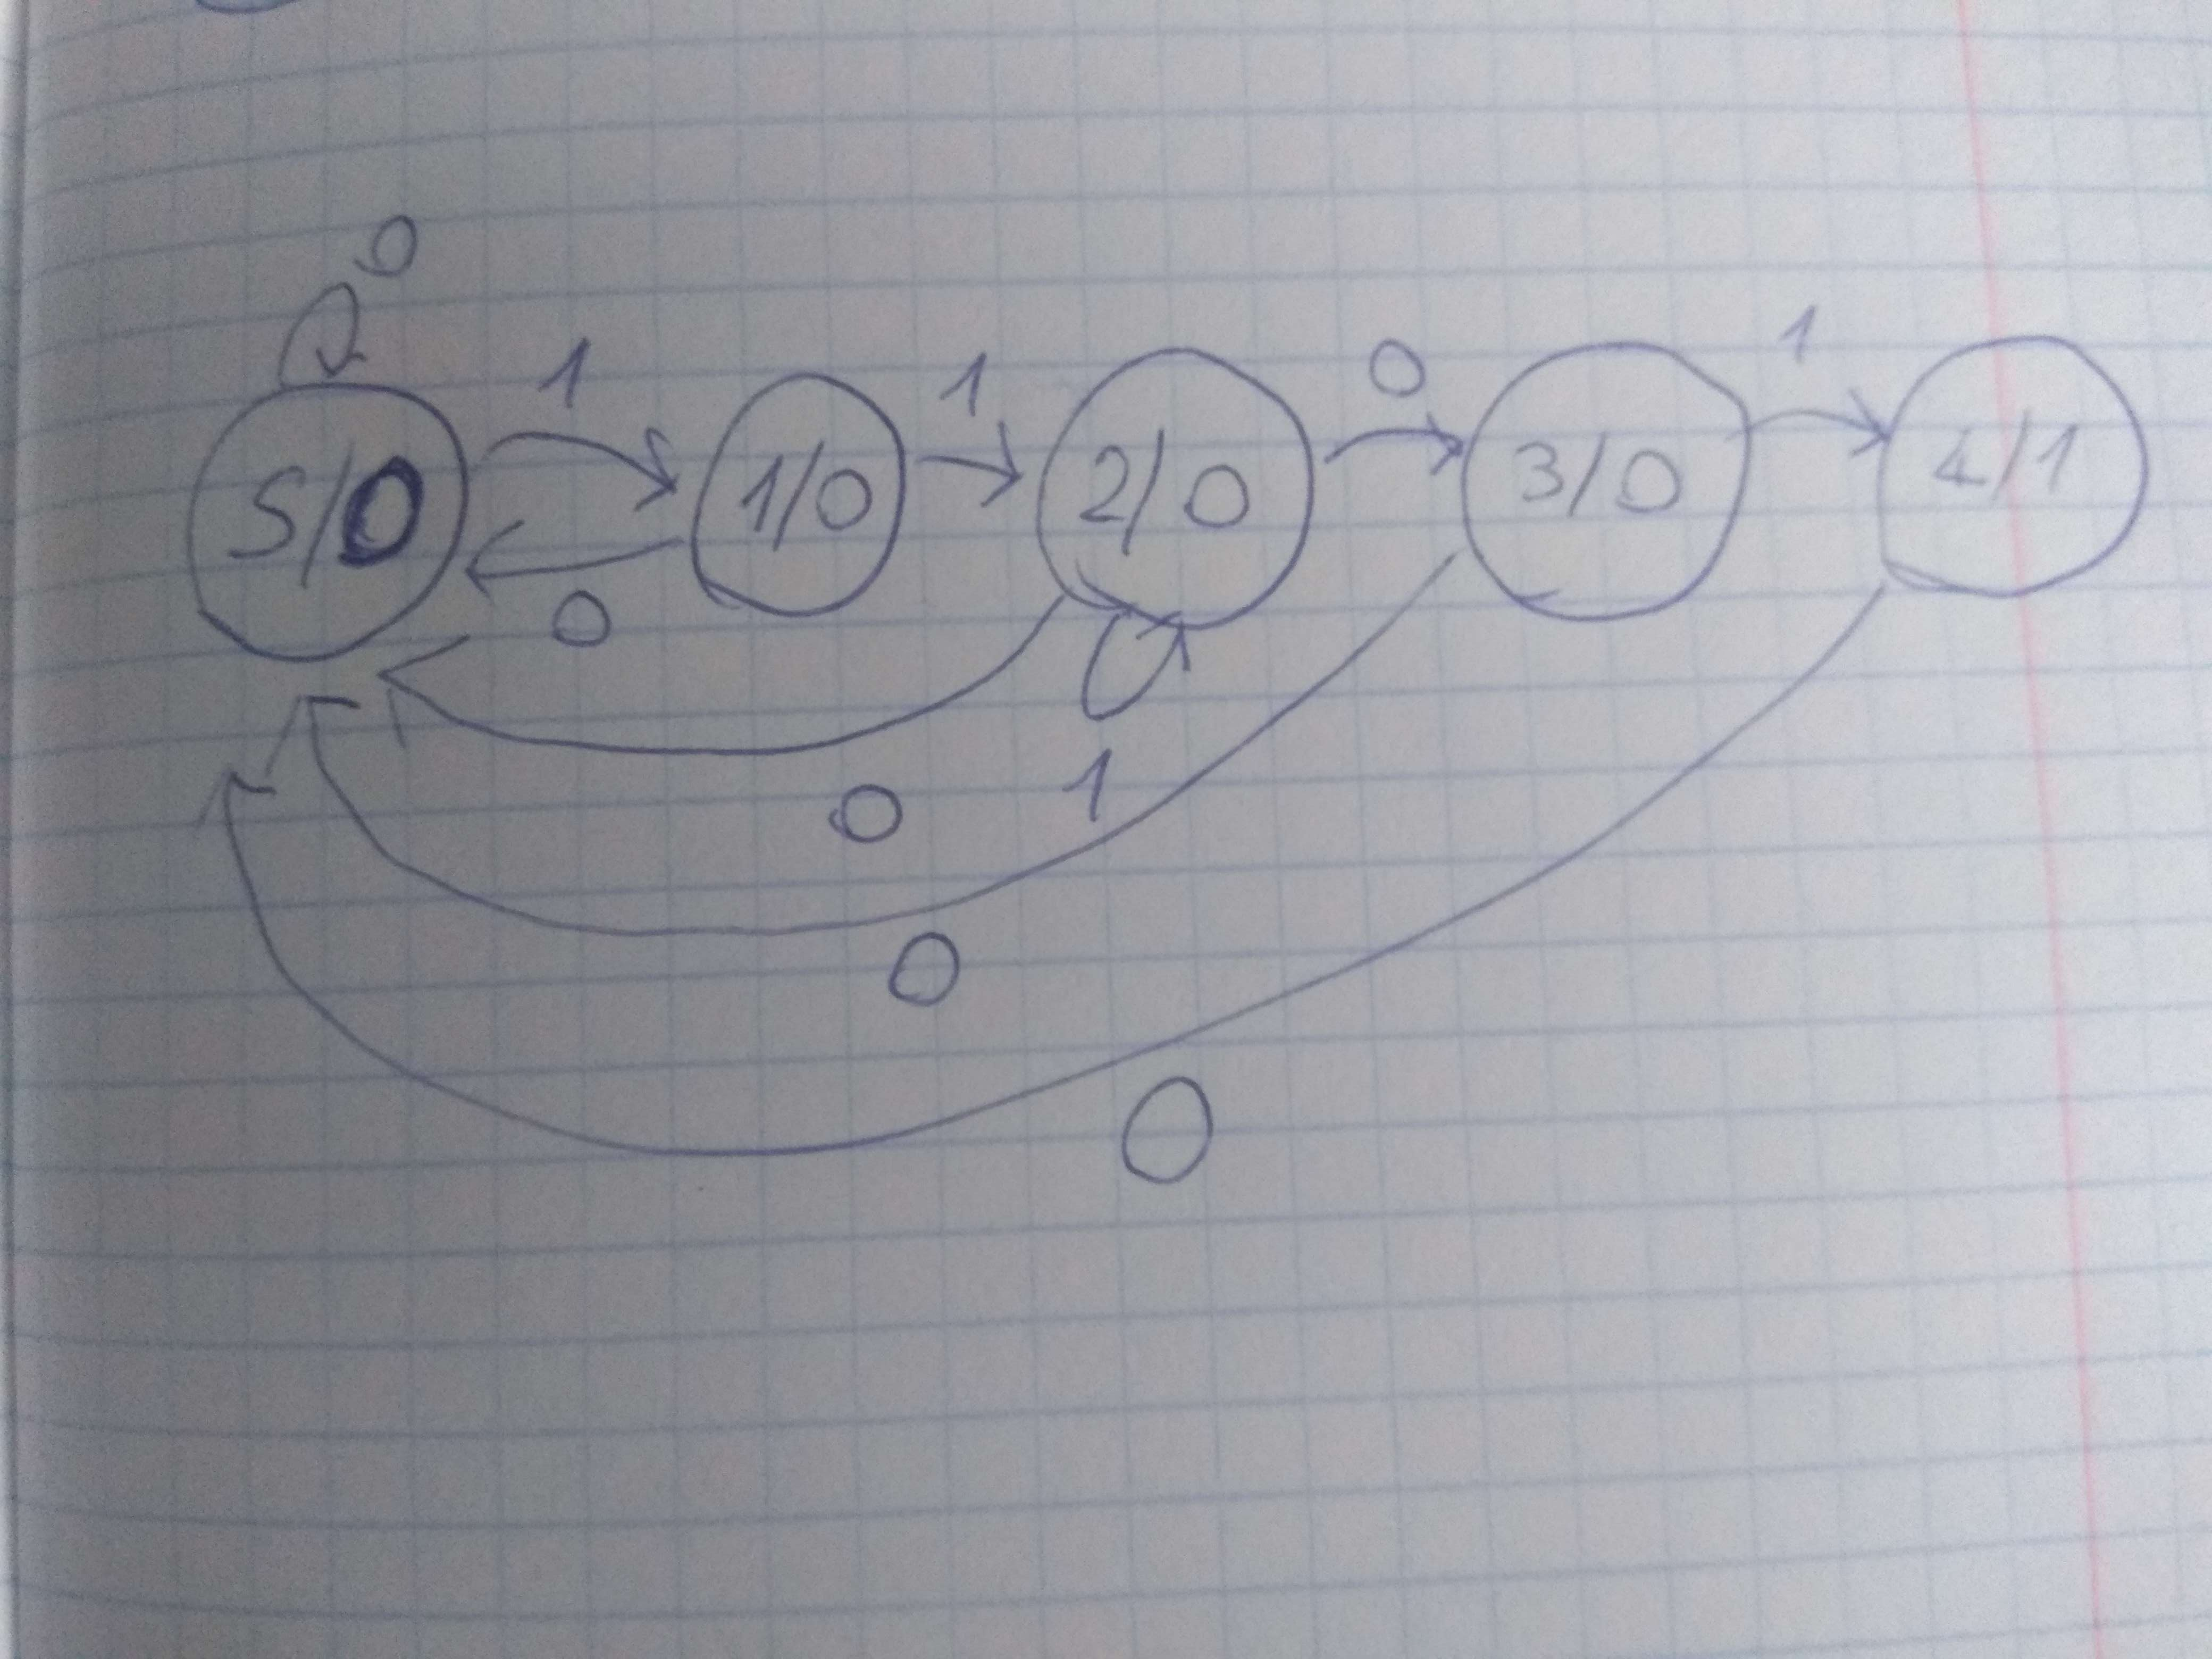
\includegraphics[width = 0.5\textwidth]{3b_automat}
\end{figure}
\subsection{Funkcje przejścia stanu}
\begin{figure}[H]
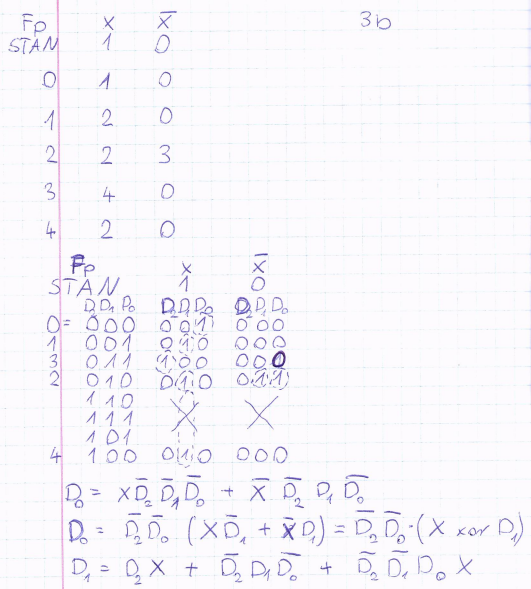
\includegraphics[width = 0.5\textwidth]{3b_przejscia}
\end{figure}
\subsection{Funkcja wyjścia}
\begin{figure}[H]
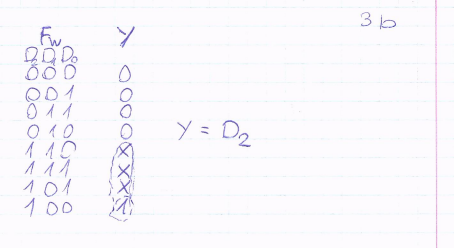
\includegraphics[width = 0.5\textwidth]{3b_wyjscia}
\end{figure}
\subsection{Schemat układu}
\begin{figure}[H]
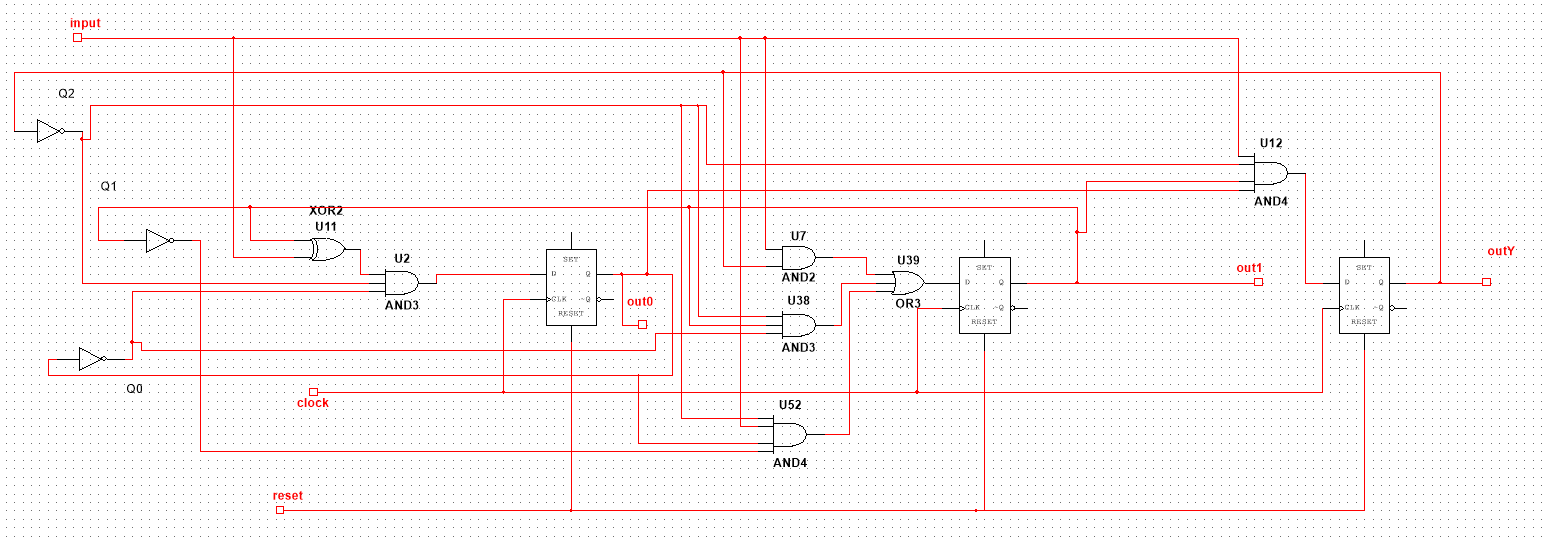
\includegraphics[width = \textwidth]{3b_uklad}
\end{figure}
W połączeniu z układem PISO:
\begin{figure}[H]
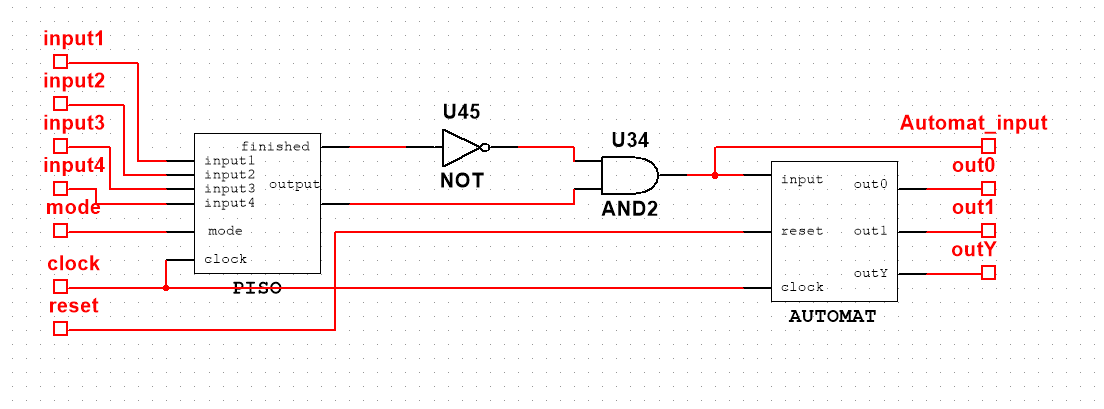
\includegraphics[width = \textwidth]{3b_uklad_z_2b_blackbox}
\end{figure}
\subsection{Układ testujący}
Przygotowaliśmy automatyczny model testujący. Lampka błędu pozostanie zgaszona tylko jeżeli we wszystkich sytuacjach licznik zachowa się zgodnie z oczekiwaniami.
\begin{figure}[H]
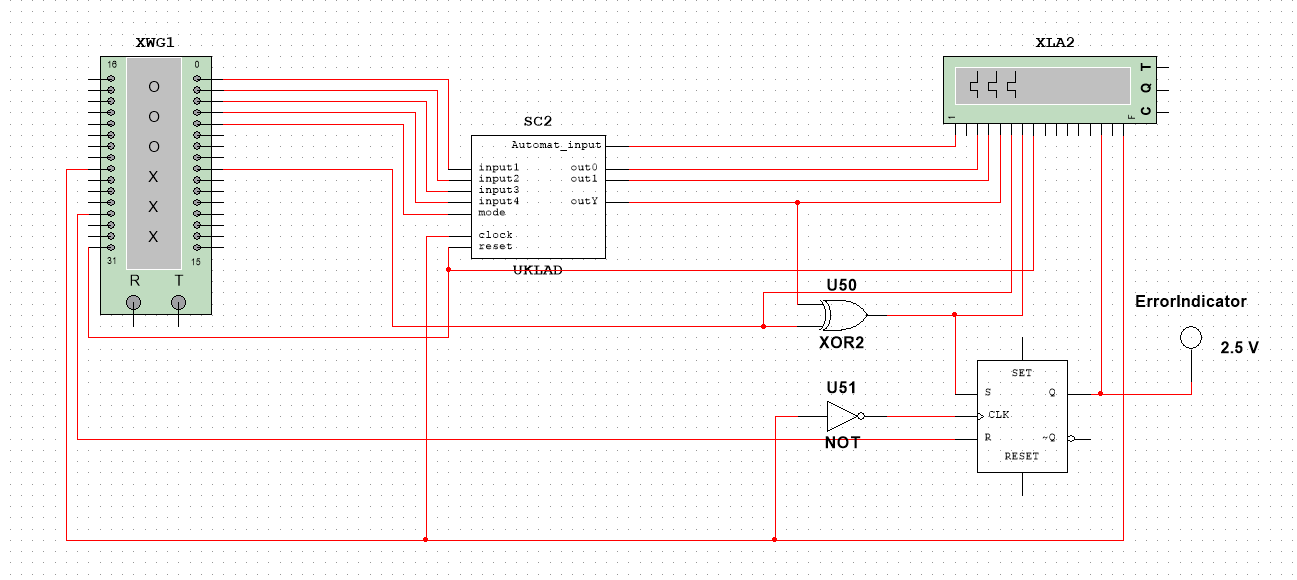
\includegraphics[width = \textwidth]{3b_tester}
\end{figure}
Załączamy kod wykorzystany do utworzenia konfiguracji generatora słów.
\begin{lstlisting}
output = []

def toBinary(val):
    res = []
    while val != 0:
        res.insert(0, val % 2)
        val = val // 2

    while len(res) < 4:
        res.insert(0, 0)
    
    return res

def hex4(val):
    res = hex(val)[2:]
    while len(res) < 4:
        res = "0" + res
    return res

def addOutput(data):
    output.append(data[:1] + '1' + data[2:])
    output.append(data[:1] + '0' + data[2:])

output.append("Data:\n")
addOutput("10000000\n") 
for i in range(16):
    addOutput("80000000\n")
    addOutput('0000001' + hex(i)[2:] + '\n')
    binary = toBinary(i)
    for k in range(4):                              
        addOutput('00000000' + '\n')
    addOutput('00000' + str(int(i == 13)) + '00' + '\n')

output.append("Initial:" + '\n')
output.append("0000" + '\n')
output.append("Final:" + '\n')
output.append(hex4(224) + '\n')

with open('output.dp', 'w') as outputFile:
    outputFile.writelines(output)
\end{lstlisting}
Rezultaty z analizatora logicznego. Linia "20" stale na 1 oznacza brak błędu.
\begin{figure}[H]
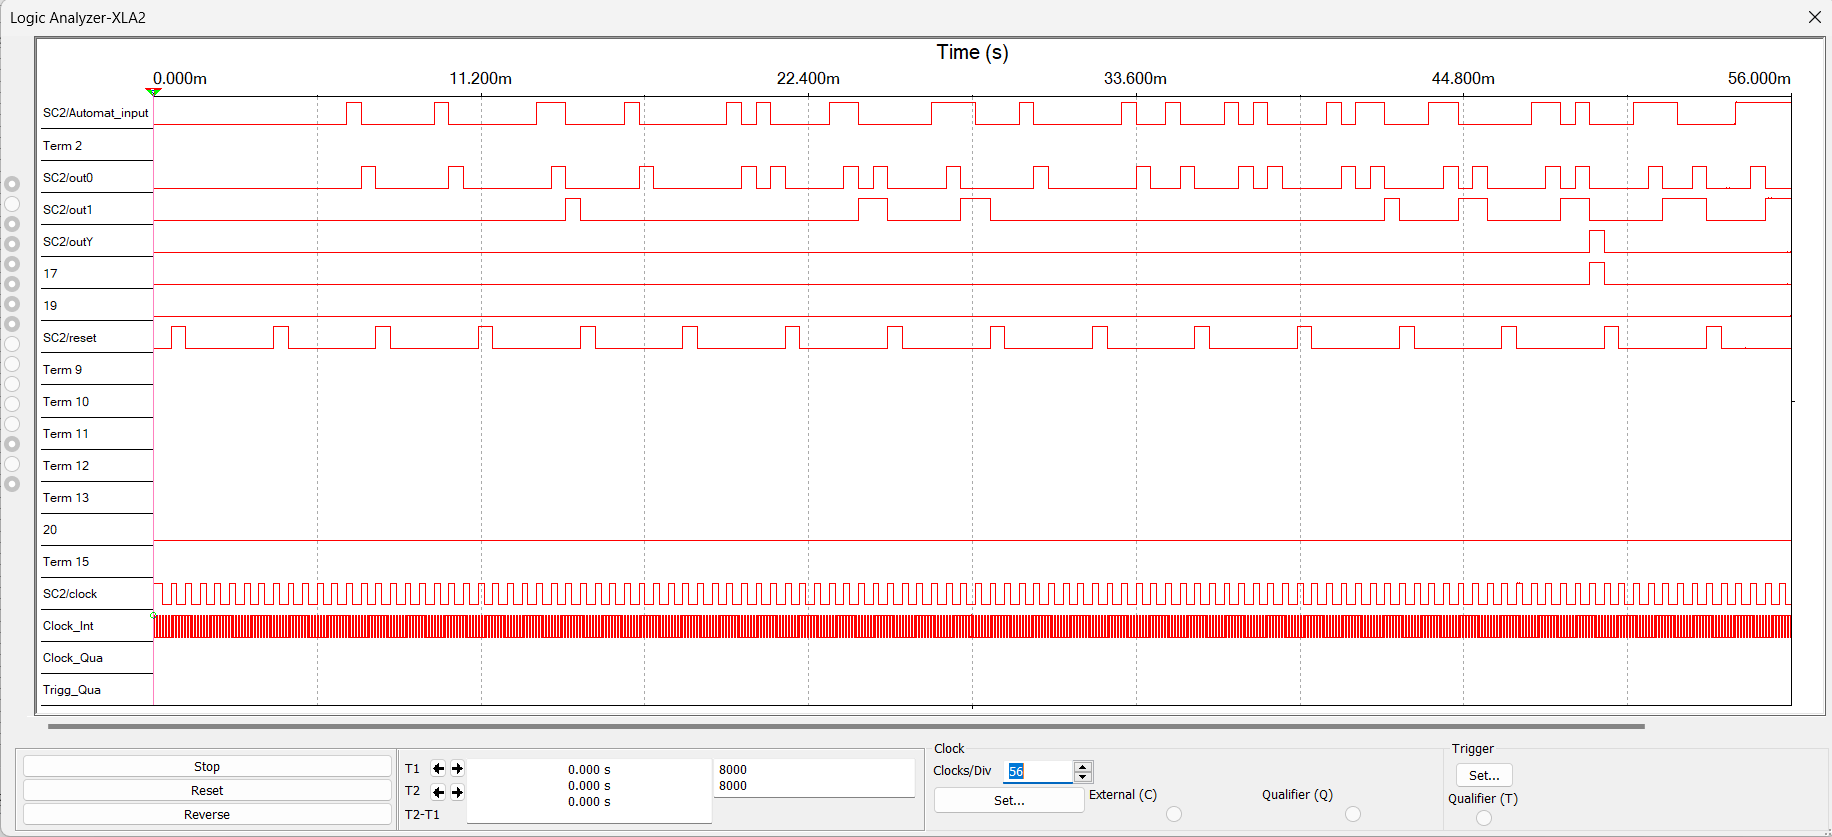
\includegraphics[width = \textwidth]{3b_analyzer}
\end{figure}
\subsection{Wnioski}
\paragraph{Alternatywne rozwiązania}
\paragraph{Zastosowania}
\end{document}